\documentclass{article}
\usepackage[utf8]{inputenc}
\usepackage{amsmath,amssymb,mathtools}
\usepackage{amsthm}
\usepackage{thmtools}
\usepackage{hyperref}
% `cleveref` has to be loaded after `hyperref`
\usepackage{cleveref}
\usepackage{stackengine}
\usepackage{minted}
\usepackage{tcolorbox}
\usepackage{multicol}
\usepackage{prftree}
\usepackage{fancyvrb}
\usepackage{csquotes}
\usepackage{appendix}

\title{Cartesian Reachability Logic}
\author{Jan Tušil }
\date{February 2022}

\declaretheorem[]{example}
\declaretheorem[]{definition}
\declaretheorem[]{lemma}
\declaretheorem[]{theorem}
\declaretheorem[]{remark}

\newcommand{\RL}{\mathsf{RL}}
\newcommand{\ML}{\mathsf{ML}}
\newcommand{\CRL}{\mathsf{CRL}}
\newcommand{\Var}{\mathit{Var}}
\newcommand{\Tcfg}{\mathcal{T}_{\mathit{Cfg}}}

\newcommand\oast{\stackMath\mathbin{\stackinset{c}{0ex}{c}{0ex}{\ast}{\bigcirc}}}

\begin{document}

\maketitle

\section{Introduction}

\section{Preliminaries}

\subsection{(Topmost, $\mu$-free) Matching Logic}

\subsection{All-path Reachability Logic}



\begin{definition}[\cite{StefanescuCMMSR19}]
We define reachability-logic signatures, rules, and systems as follows.
\begin{enumerate}
    \item A reachability-logic \emph{signature} is a pair $(\Sigma, \mathit{Cfg})$,
          where $\Sigma$ is a matching logic signature and $\mathit{Cfg}$ is a sort.
          
    \item A \emph{one-path reachability rule} over reachability logic signature $(\Sigma, \mathit{Cfg})$        is a pair $\varphi \Rightarrow^\exists \varphi^\prime$,
          where $\varphi$ and $\varphi^\prime$
          are patterns (which can have free variables) of sort $\mathit{Cfg}$.
          
    \item A \emph{reachability system} over a reachability-logic signature $(\Sigma, \mathit{Cfg})$
          is a pair $\mathcal{S} = (\mathcal{T}, S)$, where $\mathcal{T}$ is a $\Sigma$-algebra
          and $S$ is a set of reachability rules over $(\Sigma, \mathit{Cfg})$.
          
    \item A rule $\varphi \Rightarrow^\exists \varphi^\prime$ over $(\Sigma, \mathit{Cfg})$
          is \emph{weakly well-defined}
          with respect to $\Sigma$-algebra $\mathcal{T}$
          iff
          for any $\gamma \in \Tcfg$ and $\rho : \Var \to \mathcal{T}$
          with $(\gamma, \rho) \vDash \varphi$,
          there exists $\gamma^\prime \in \Tcfg$ with $(\gamma^\prime , \rho) \vDash \varphi^\prime$.
          
    \item A reachability system $\mathcal{S}$ is \emph{weakly well-defined} iff each its rule is weakly     
          well-defined.
          
    \item A reachability system $\mathcal{S} = (\mathcal{T}, S)$ over $(\Sigma, \mathit{Cfg})$ induces
          a \emph{transition system} \\
          $(\Tcfg , \Rightarrow_{\mathcal{S}})$,
          where $\gamma \Rightarrow_{\mathcal{S}} \gamma^\prime$
          for $\gamma, \gamma^\prime \in \Tcfg$
          iff there is some rule \\ $\varphi \Rightarrow^\exists \varphi^\prime \in S$
          and some valuation $\rho : \Var \to \mathcal{T}$ with $(\gamma, \rho) \vDash \varphi$
          and $(\gamma^\prime , \rho) \vDash \varphi^\prime$.
          
    \item A \emph{$\Rightarrow_{\mathcal{S}}$-path} is a finite
          sequence $\gamma_0 \Rightarrow_{\mathcal{S}} \gamma_1 \Rightarrow_{\mathcal{S}} \ldots \Rightarrow_{\mathcal{S}} \gamma_n$
          with $\gamma_0,\ldots,\gamma_n \in \Tcfg$.
          
    \item A $\Rightarrow_{\mathcal{S}}$-path is \emph{complete}
          iff it is not a strict prefix of any
          other $\Rightarrow_{\mathcal{S}}$-path.

    \item An \emph{all-path reachability rule}
          is a pair $\varphi \Rightarrow^\forall \varphi^\prime$ of patterns $\varphi$ and $\varphi^\prime$.
    
    \item An all-path reachability rule $\varphi \Rightarrow^\forall$ is \emph{satisfied},
          written $\mathcal{S} \vDash_\RL \varphi \Rightarrow^\forall \varphi^\prime$,
          iff for all complete $\Rightarrow_{\mathcal{S}}$-paths $\tau$
          starting with $\gamma \in \Tcfg$ and for all $\rho : \Var \to \mathcal{T}$
          such that $(\gamma, \rho) \vDash \varphi$,
          there exists some $\gamma^\prime \in \tau$
          such that $(\gamma^\prime, \rho) \vDash \varphi^\prime$.
\end{enumerate}

\begin{figure}
    \centering
    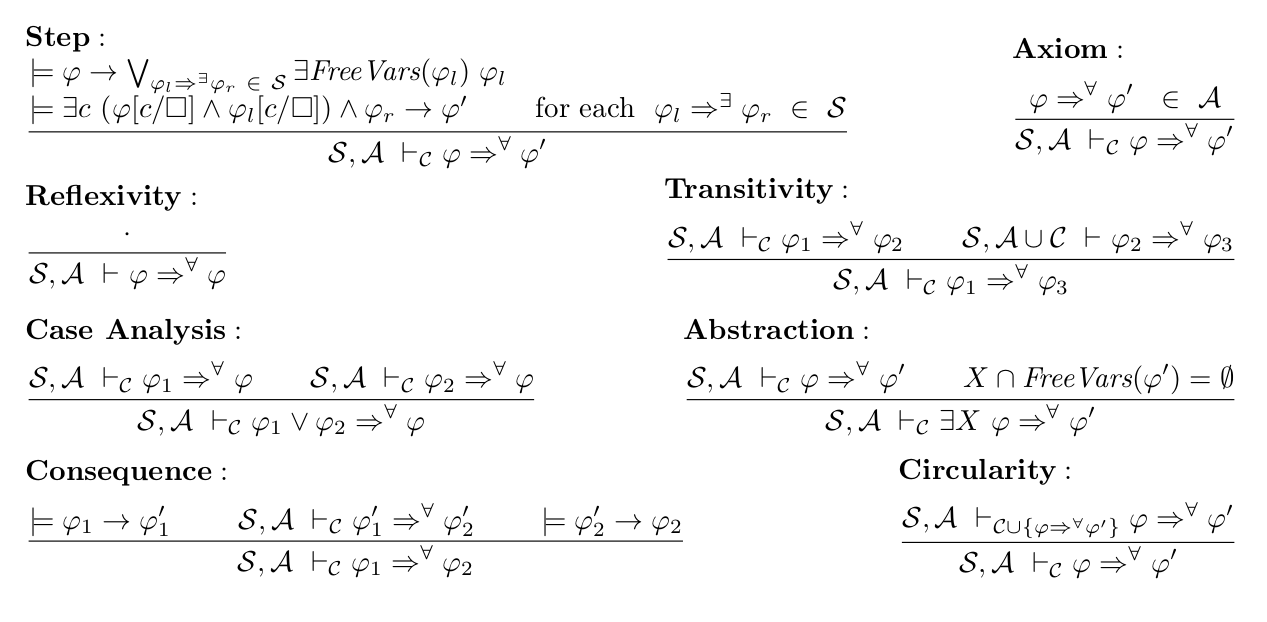
\includegraphics[width=0.9\textwidth]{img/rl-proofsystem.png}
    \caption{All-path reachability-logic proof system. TODO retypeset}
    \label{fig:RLproofsystem}
\end{figure}

TODO proof system

We have RL sequents of the shape $\mathcal{S}, A, C \vdash_\RL \varphi \Rightarrow^\forall \varphi^\prime$.

\end{definition}

\section{Cartesian Reachability Logic}

We need to make the definition such that it works with reachability logic for the composite semantics.
Here is one attempt:
\begin{definition}\label{def:CRLsemantics}
A Cartesian reachability rule
$(\varphi_1,\ldots,\varphi_k) \land \varphi \Rightarrow^{c\forall} (\psi_1,\ldots,\psi_k) \land \psi$
of arity $k$
is \emph{valid},
written
$\vDash_\CRL (\varphi_1,\ldots,\varphi_k) \land \varphi \Rightarrow^{c\forall}
(\psi_1,\ldots,\psi_k) \land \psi$,
iff for all configurations $\sigma_1,\ldots,\sigma_k$ and any valuation $\rho$,
whenever $\sigma_1 \in |\varphi_1 \land \varphi|_\rho \land \ldots \land \sigma_k \in |\varphi_l \land \varphi|_\rho$,
then for every complete (that is, finite terminating) executions $\pi_1, \ldots, \pi_k$ such that
$\sigma_1 = \pi_1(0) \land \ldots \land \sigma_k = \pi_k(0)$ there exists $i_1,\ldots,i_k \in \mathbb{N}$
such that
$\pi_1(i_1) \in |\varphi_1 \land \psi|_\rho \land \ldots \land \pi_k(i_k) \in |\varphi_k \land \psi|_\rho$.
\end{definition}

TODOs:
\begin{itemize}
    \item Validate this definition against examples from the CHL paper.
    \item Have a "running example" - some programming language, like IMP?
    \item Define the 'composite' semantics - list of configurations in one configuration.
    \item Have an example how do we perform lockstep execution on ifs.
    \item Why there are the pluses on both premises of the Circularity proof rule of the Equiv checking paper? Do we need it? Maybe we may lose/miss some synchronization point if we require both. We probably need to weaken the premises.
    \item Conservativeness argument for the additional rules.
\end{itemize}

\begin{definition}
We translate a language semantics into a semantics for lists of configurations as follows.
\begin{enumerate}
    \item Let $(\Sigma, \mathit{Cfg})$ be a reachability-logic signature.
          Then $(\Sigma, \mathit{Cfg})^*$ = $(\Sigma^*, \mathit{Cfg}^*)$,
          where
          \begin{enumerate}
              \item $\Sigma^* = \Sigma \cup \{ \mathit{cfgitem}, \mathit{cfgconcat},
          %\mathit{cfgdummy},
          \mathit{cfgheat} \}$
              \item $\mathit{Cfg}^*$ is a fresh sort (representing the sort of lists of configurations);
              %\item $\mathit{cfgdummy}$ is a fresh symbol of sort $\mathit{Cfg}$;
              \item $\mathit{cfgitem}$ a fresh symbol of sort $\mathit{Cfg} \to \mathit{Cfg}^*$;
              \item $\mathit{cfgconcat}$ a fresh symbol of sort $\mathit{Cfg}^* \times \mathit{Cfg}^* \to \mathit{Cfg}^*$; and
              \item $\mathit{cfgheat}$ is a fresh symbol of sort $\mathit{Cfg}^* \times \mathit{Cfg} \times \mathit{Cfg}^* \to \mathit{Cfg}^*$.
          \end{enumerate}
    \item Let $S$ be a set of reachability rules over $(\Sigma, \mathit{Cfg})$.
          We generate a set of reachability rules $S^*$ over $(\Sigma, \mathit{Cfg})^*$
          by setting
          \begin{equation*}
              S^* = \{ \mathit{cfgheat}(L, \varphi_1, R) \land P \Rightarrow^\exists \mathit{cfgheat}(L, \varphi_2, R) \land P^\prime \mid (\varphi_1 \land P \Rightarrow^\exists \varphi_2 \land P^\prime) \in S \} \, ,
          \end{equation*}
          where $L,R$ are distinct fresh variables (not occurring in any rule in $S$).
    \item Let $\mathcal{T}$ be a configuration model; that is, a $\Sigma$-algebra.
          We generate a $\Sigma^*$-algebra $\mathcal{T}*$, which interprets all sorts and symbols from
          $\Sigma$ as in $\mathcal{T}$, and in addition interprets
          \begin{enumerate}
              \item the sort $\mathit{Cfg}*$ as the set of all finite lists
              $[c_1;\ldots;c_n]$ for $n \in \mathbb{N}$, where $c_i$ is an element of sort $\mathit{Cfg}$
              for any $0 \leq i \leq n$;
              \item the symbol $\mathit{cfgitem}$ as the function $\lambda c.\, [c]$;
              \item the symbol $\mathit{cfgconcat}$ as the function $\lambda l_1,l_2.\, l_1 \texttt{++} l_2$,
                where $\texttt{++}$ is list concatenation; and
              \item the symbol $\mathit{cfgheat}$ as the function
                $\lambda l_1, c, l_2.\, l_1 \texttt{++} [c] \texttt{++} l_2$.
          \end{enumerate}
          
    \item Let $\mathcal{S} = (\mathcal{T}, S)$ be a reachability system over $(\Sigma, \mathit{Cfg})$.
          We generate a reachability system $\mathcal{S}^*$ over $(\Sigma, \mathit{Cfg})^*$
          by setting $\mathcal{S}^* = (\mathcal{T}^*, S^*)$.
\end{enumerate}
\end{definition}

\begin{lemma}
    Let $\mathcal{S} = (\mathcal{T}, S)$ be a reachability-logic system over $(\Sigma, \mathit{Cfg})$.
    For any $k \geq 1$, any configurations $c_1,\ldots,c_k, c^\prime \in \Tcfg$, and any $1 \leq i \leq k$,
    we have
    \begin{equation*}
        c_i \Rightarrow_{\mathcal{S}} c^\prime
                    \iff
        [c_1,\ldots,c_k] \Rightarrow_{\mathcal{S}^*} [c_1, \ldots, c_{i-1}, c^\prime, c_{i+1}, \ldots, c_k]
    \end{equation*}
\end{lemma}
\begin{proof}
Admitted.
\end{proof}


\section{Proof System}

The proof system derives claims of the shape
$\vdash_\CRL (\varphi_1 \land P_1, \ldots, \varphi_k \land P_k) \land P \Downarrow_C E$,
where $\varphi_i$ are structural patterns, and $P_i$ and $P$ are predicate patterns.
Maybe we need a constraint that $\mathit{FV}(P_i) \subseteq \mathit{FV}(\varphi_i)$.
That way we can feed the $(\varphi_i, P_i)$ component to RL without some unexpected behavior.
The idea is that $P$ is the part of the claim that relates variables from different components.
Therefore, we also probably need the Consequence rule to work with $P$, too.

\begin{definition}
We define $\mathit{mergePatterns}$ and $\mathit{flatten}$ as follows:
\begin{enumerate}
    \item $\mathit{mergePatterns}(\varphi) = \mathit{cfgitem}(\varphi)$;
    \item $\mathit{mergePatterns}(\varphi_1, \varphi_2, \ldots, \varphi_n)
        = \mathit{cfgconcat}(\mathit{cfgitem}(\varphi_1), \mathit{mergePatterns}(\varphi_2, \ldots, \varphi_n))$ for $n \geq 2$; and
    \item $\mathit{flatten}((\varphi_1 \land P_1, \ldots, \varphi_k \land P_k) \land P)
           = \mathit{mergePatterns}(\varphi_1, \ldots, \varphi_k) \land (P_1 \land \ldots \land P_k \land P)$.
    \item $\mathit{flatten}^\prime(\psi, \psi^\prime) = \mathit{flatten}(\psi) \Rightarrow^\forall \mathit{flatten}(\psi^\prime)$
    \item $\mathit{flatten}^\prime(A, \psi^\prime) = \{ \mathit{flatten}^\prime(\psi, \psi^\prime) \mid \psi \in A \}$, where $A$ is a set.
\end{enumerate}
\end{definition}

\begin{figure}
    \centering
    \begin{align*}
    & \prftree[l]{Reflexivity}{\mathcal{S} \vdash_\CRL \psi \Downarrow_{\emptyset,E} \psi}
    \end{align*}
    \begin{align*}
    & \prftree[l]{Axiom}{\psi \in E}{\mathcal{S} \vdash_\CRL \psi \Downarrow_{C,E} \psi^\prime}
    \end{align*}
    \begin{align*}
    & \prftree[l]{Reduce}
      {\mathcal{S}^*, \mathit{flatten}^\prime(E, \psi^\prime), \emptyset \vdash_\RL
        \mathit{flatten}^\prime(\psi, \psi^\prime) }
      {\mathcal{S} \vdash_\CRL \psi \Downarrow_{C,E} \psi^\prime}
    \end{align*}
    \begin{align*}
    & \prftree[l]{Case}
    { \prfStackPremises
      {\mathcal{S} \vdash_\CRL (\varphi_1, \ldots, \varphi_{i-1}, \varphi_i \land P, \varphi_{i+1}, \ldots, \varphi_k) \land P^\prime \Downarrow_{C, E} \psi^\prime }
      {\mathcal{S} \vdash_\CRL (\varphi_1, \ldots, \varphi_{i-1}, \varphi_i \land Q, \varphi_{i+1}, \ldots, \varphi_k) \land P^\prime \Downarrow_{C, E} \psi^\prime }
    }
    {\mathcal{S} \vdash_\CRL (\varphi_1, \ldots, \varphi_{i-1}, \varphi_i \land (P \lor Q), \varphi_{i+1}, \ldots, \varphi_k) \land P^\prime \Downarrow_{C, E} \psi^\prime}
    \end{align*}
    \begin{align*}
    & \prftree[l]{Step}
    { \prfStackPremises
       %{ \mathcal{S}^* \vDash_\RL \varphi_i \Rightarrow^{\forall+} \varphi_i^\prime }
       {  (\mathcal{T}, S) \vdash_\CRL (\varphi_1, \ldots, \varphi_{i-1}, \varphi_i^\prime, \varphi_{i+1}, \ldots,    \varphi_k)
          \land P
          \Downarrow_{\emptyset, (C \cup E)} \psi^\prime
      }
      { \mathcal{T} \vDash_{\ML} \varphi_i \rightarrow \bigvee \{ \exists \mathit{FV}(\varphi_l).\, \varphi_l \mid \varphi_l \Rightarrow^\exists \varphi_r \in S \} }
      { \mathcal{T} \vDash_\ML ((\exists c.\, \varphi_i[c/\square] \land \varphi_l[c/\square]) \land \varphi_r) \rightarrow \varphi_i^\prime  \mbox{ for each } \varphi_l \Rightarrow^\forall \varphi_r \in S }
    }
    {\mathcal{S} \vdash_\CRL (\varphi_1, \ldots, \varphi_{i-1}, \varphi_i, \varphi_{i+1}, \ldots, \varphi_k) \land P \Downarrow_{C, E} \psi^\prime}
    \end{align*}
    \begin{align*}
    & \prftree[l]{Circularity}
      { \mathcal{S} \vdash_\CRL (\varphi_1, \ldots, \varphi_k) \land P \Downarrow_{C \cup \{ (\varphi_1, \ldots, \varphi_k) \land P \} , E} \psi^\prime}
      { \mathcal{S} \vdash_\CRL (\varphi_1, \ldots, \varphi_k) \land P \Downarrow_{C, E} \psi^\prime}
    \end{align*}
    \begin{align*}
    & \prftree[l]{Conseq}
      { \prfStackPremises
        { (\mathcal{T}, S) \vdash_\CRL (\varphi_1 \land P_1, \ldots, \varphi_k \land P_k) \land P \Downarrow_{C, E} \psi^\prime}
        { \mathcal{T} \vDash_\ML \varphi_1 = \varphi_1^\prime \land \ldots \land \varphi_k = \varphi_k^\prime
        \land (P_1 \land \ldots \land P_k \land P \leftrightarrow P_1 \land \ldots \land P_k \land P) }
      }
      { (\mathcal{T}, S) \vdash_\CRL (\varphi_1^\prime \land P_1^\prime, \ldots, \varphi_k^\prime \land P_k^\prime) \land P^\prime \Downarrow_{C, E} \psi^\prime}
    \end{align*}
    \caption{Proof System}
    \label{fig:my_label}
\end{figure}



\begin{lemma}
    \begin{equation*}
        \mathcal{S} \vdash_\CRL \psi \Downarrow_{C,E} \psi^\prime
        \implies
        \mathcal{S}^*, \mathit{flatten}^\prime(E, \psi^\prime), \mathit{flatten}^\prime(C, \psi^\prime) \vdash_\RL
          \mathit{flatten}^\prime(\psi, \psi^\prime) 
    \end{equation*}
\end{lemma}
\begin{proof}
By induction on the structure of the CRL proof. TODO
\begin{enumerate}
    \item If the proof ends with \emph{Reduce}, then we are done, since $\mathit{flatten}^\prime(\emptyset, \psi^\prime) = \emptyset$.
    
    \item If the proof ends with \emph{Reflexivity}, then we need to prove
    \begin{equation*}
        \mathcal{S}^*, \mathit{flatten}^\prime(E, \psi), \emptyset \vdash_\RL
          \mathit{flatten}^\prime(\psi, \psi) 
    \end{equation*}
    which we do by applying the Reflexivity proof rule.
    
    \item If the proof ends with \emph{Axiom}, then $\psi \in E$,
          and we have to prove that
          \begin{equation*}
            \mathcal{S}^*, \mathit{flatten}^\prime(E, \psi^\prime), \mathit{flatten}^\prime(C, \psi^\prime) \vdash_\RL
            \mathit{flatten}^\prime(\psi, \psi^\prime)               \, .
          \end{equation*}
          By applying the Axiom proof rule of RL, it is enough to show that
          \begin{equation*}
              \mathit{flatten}^\prime(\psi, \psi^\prime) \in \mathit{flatten^\prime}(E, \psi^\prime) \, ,
          \end{equation*}
          which follows from $\psi \in E$.
          
    \item If the proof ends with \emph{Case}, then we have
        \begin{equation*}
            \mathcal{S}^*, \Bar{E}, \Bar{C} \vdash_\RL
            \mathit{flatten}^\prime((\varphi_1, \ldots, \varphi_{i-1}, \varphi_i \land P, \varphi_{i+1}, \ldots, \varphi_k) \land P^\prime, \psi^\prime)
        \end{equation*}
        and
        \begin{equation*}
            \mathcal{S}^*, \Bar{E}, \Bar{C} \vdash_\RL
            \mathit{flatten}^\prime((\varphi_1, \ldots, \varphi_{i-1}, \varphi_i \land Q, \varphi_{i+1}, \ldots, \varphi_k) \land P^\prime, \psi^\prime) 
        \end{equation*}
        as hypotheses, and we have to prove
        \begin{equation*}
            \mathcal{S}^*, \Bar{E}, \Bar{C} \vdash_\RL
            \mathit{flatten}^\prime((\varphi_1, \ldots, \varphi_{i-1}, \varphi_i \land (P \lor Q), \varphi_{i+1}, \ldots, \varphi_k) \land P^\prime, \psi^\prime)               \, .
        \end{equation*}
        (where $\Bar{E} = \mathit{flatten}^\prime(E, \psi^\prime)$
         and $\Bar{C} = \mathit{flatten}^\prime(C, \psi^\prime)$
        )
        We split every $\varphi_j$ into its structural part $\phi_j$ and a predicate part $P_j$,
        which allows us to simplify the instances of $\mathit{flatten}^\prime$.
        This gives us the hypotheses
         \begin{align*}
            \mathcal{S}^*, \Bar{E}, \Bar{C}
            \vdash_\RL
            & \mathit{mergePatterns}(\phi_1, \ldots, \phi_k)
            \\ & \land (P_1 \land \ldots \land P_{i-1} \land P \land P_{i+1} \land \ldots \land P_k \land P^\prime) 
            \\ & \Rightarrow^\forall \mathit{flatten}(\psi^\prime) 
        \end{align*}
        and
        \begin{align*}
            \mathcal{S}^*, \Bar{E}, \Bar{C}
            \vdash_\RL
            & \mathit{mergePatterns}(\phi_1, \ldots, \phi_k)
            \\ & \land (P_1 \land \ldots \land P_{i-1} \land Q \land P_{i+1} \land \ldots \land P_k \land P^\prime) 
            \\ & \Rightarrow^\forall \mathit{flatten}(\psi^\prime) \, ,
        \end{align*}
        and the goal to prove will be
        \begin{align*}
            \mathcal{S}^*, \Bar{E}, \Bar{C}
            \vdash_\RL
            & \mathit{mergePatterns}(\phi_1, \ldots, \phi_k)
            \\ & \land (P_1 \land \ldots \land P_{i-1} \land (P \lor Q) \land P_{i+1} \land \ldots \land P_k \land P^\prime) 
            \\ & \Rightarrow^\forall \mathit{flatten}(\psi^\prime) \, .
        \end{align*}
        Now we apply the Consequence RL rule on the goal, changing it to
        \begin{align*}
            \mathcal{S}^*, \Bar{E}, \Bar{C}
            \vdash_\RL
            & (\mathit{mergePatterns}(\phi_1, \ldots, \phi_k)
            \\ & \quad \land (P_1 \land \ldots \land P_{i-1} \land P \land P_{i+1} \land \ldots \land P_k
            \land P^\prime))
            \\ & \lor (\mathit{mergePatterns}(\phi_1, \ldots, \phi_k)
            \\ & \quad \land (P_1 \land \ldots \land P_{i-1} \land Q \land P_{i+1} \land \ldots \land P_k
            \land P^\prime))
            \\ & \Rightarrow^\forall \mathit{flatten}(\psi^\prime) \, .
        \end{align*}
        Now we apply the Case analysis RL rule and the hypotheses and we are done.
\end{enumerate}
\end{proof}

\section{Implementation}

\bibliography{bibliography}
\bibliographystyle{plain}

\appendix


\end{document}
